\documentclass[10pt,a4paper]{article}
\usepackage[a4paper,margin=1.7cm,top=1.5cm,bottom=1.6cm]{geometry}
\usepackage{mathpazo}
\usepackage{amsmath,amssymb}
\usepackage{graphicx,booktabs,enumitem,xcolor,url}
\usepackage[compact]{titlesec}
\usepackage[font=small,labelfont=bf,skip=3pt]{caption}
\titleformat{\section}{\normalsize\bfseries\color[HTML]{1F3A68}}{\thesection}{0.5em}{}
\titlespacing*{\section}{0pt}{6pt}{2pt}
\setlist{itemsep=1pt,topsep=2pt,parsep=0pt,leftmargin=1.2em}
\setlength{\parskip}{2pt}\setlength{\parindent}{0pt}
\definecolor{adj}{HTML}{2A78D6}\definecolor{pinn}{HTML}{EB6834}\definecolor{joint}{HTML}{14855C}
\urlstyle{same}
\begin{document}
\begin{center}
{\large\bfseries IE 643 Course Project --- Novelty Assessment Report}\\[2pt]
{\bfseries PINN-Based Inverse Estimation of Spatially Varying Diffusion Coefficients}\\[2pt]
Team \textbf{Binary\_Brains}: Jash Taparia (24B2451, 24b2451@iitb.ac.in), Mihir Gune (24B2443, 24b2443@iitb.ac.in)\\
Code: \url{https://github.com/bloodrepaer/IE643-Binary-Brains-PINN-Inversion}
\end{center}
\vspace{-4pt}

\section{Problem and what the novelty phase set out to do}
We recover $D(x,y)$ in $u_t=\nabla\!\cdot\!(D\nabla u)+f$ on $[0,1]^2$ from noisy readings
$d_k=u(x_k,y_k,t_k)+\varepsilon_k$, $\varepsilon_k\sim\mathcal N(0,\sigma^2)$. \textbf{Known:} the initial state $u_0$, the
noise level $\sigma$ and, in the standard setting, the wall temperature $g$ and source $f$. \textbf{Measured:} $d_k$ at
5--3\,969 sensors and 1--200 times, 0--10\,\% noise. \textbf{Estimated:} the full field $D$ (and, in the
unknown-physics setting, also $g$ or $f$). Data come from our RK4 solver on $129^2$; all inversions use $65^2$.
In the intensive phase the \textcolor{adj}{\textbf{classical adjoint}} beat the \textcolor{pinn}{\textbf{PINN}} with
known physics, while the PINN looked better with unknown physics and against a backward-Euler adjoint at high sensor
density. Following the instructor's feedback, the novelty phase (i) compares the PINN with a
\textbf{Crank--Nicolson (CN) adjoint on exactly the same observations, grids, source and boundary settings};
(ii) proposes and tests a \textbf{combined method} against both standalone methods; (iii) runs a
\textbf{controlled solver comparison}; and (iv) reports full recovered fields, spatial error maps and replay, not
only sensor fit.

\section{Approaches tried}
\begin{itemize}
\item \textcolor{joint}{\textbf{Combined PINN$\leftrightarrow$adjoint (4 couplings).}} \emph{hybrid\_path}: project the
PINN's $\log D$ onto the adjoint's $16\times16$ controls and start L-BFGS-B there, same $\alpha$ path and discrepancy
rule; \emph{hybrid\_balance}: same start, but begin the $\alpha$ path at weak regularisation so the start is not
washed out; \emph{hybrid\_prior}: Tikhonov towards the PINN field instead of towards smoothness; \emph{reverse}:
adjoint answer as the PINN's initial $D$-net.
\item \textcolor{joint}{\textbf{Joint classical inversion for unknown physics.}} The adjoint also estimates the
hidden wall temperatures (each wall uniform in space, piecewise linear in time, 17 knots) or a hidden heat source $f\ge0$ on $16\times16$ controls, with exact
discrete-adjoint gradients (checked against finite differences: $2.7\cdot10^{-7}$ for $D$, $2.6\cdot10^{-9}$ for $f$).
This gives the classical method the same freedom the PINN gets from its soft physics.
\item \textbf{Controlled solver comparison (Study 5).} The same adjoint, data and regularisation with CN or backward
Euler (BE) time stepping at 100--4\,800 steps over 50--3\,969 sensors and 1--10\,\% noise, plus a causal test: BE on
data generated by BE itself.
\item \textbf{Sensor density and training budget.} 20--3\,969 sensors for both methods; PINN at 1.5k, 6k and 24k epochs;
an exact-$u$ PINN $D$-step to separate fitting error from identifiability.
\item \textbf{PINN improvements and model error.} Held-out sensor validation for model selection, residual-based
adaptive refinement (RAR), a learned $g(u)$ for temperature-dependent $D$, pseudo-data augmentation, and an
Arrhenius family $D(x,y)\,e^{S(u-\bar u)}$ (16 datasets) where both methods face model error.
\end{itemize}
\textbf{Protocol.} 20 benchmark datasets (all six $D$ families, varied density, noise, layout and timing),
8 hidden-wall and 6 hidden-source datasets; PINN seeds 42--46; a method ``beats'' another only if its error is
more than 1\,\% lower. Metrics: rel$L_2(D)=\lVert\hat D-D\rVert/\lVert D\rVert$ (needs the truth) and replay
RMS$/\sigma$ (re-simulate $\hat D$ with CN and compare with the readings; $\approx1$ means the data are explained to the
noise level).

\section{Results}
\begin{center}
\small
\begin{tabular}{lccc}
\toprule
Median rel$L_2(D)$ (replay RMS$/\sigma$) & known physics (20) & hidden walls (8) & hidden source (6)\\
\midrule
\textcolor{adj}{\textbf{CN adjoint}} (assumes the benchmark physics) & \textbf{0.226} (0.97) & 4.36 (15.0) & 3.29 (0.99)\\
\textcolor{pinn}{\textbf{PINN}} (seed 42; 5 seeds: 0.468--0.554) & 0.468 (3.56) & 0.338 (2.48) & 0.534 (5.63)\\
\textcolor{joint}{\textbf{combined}} PINN$\to$adjoint (hybrid\_balance) & \textbf{0.225} (0.96) & 0.296 (0.92) & 3.57 (0.99)\\
\textcolor{joint}{\textbf{joint classical}} ($D$ + walls / $D$ + source) & -- & \textbf{0.264} (0.98) & \textbf{0.169} (0.97)\\
true-physics bound & -- & 0.201 & 0.156\\
\bottomrule
\end{tabular}
\captionof{table}{Same observations, grid, source and boundary settings for every method. For hidden walls the
``combined'' entry is the joint inversion started from the PINN's walls.}
\end{center}
\vspace{-6pt}
\noindent\begin{minipage}{\linewidth}
\centering
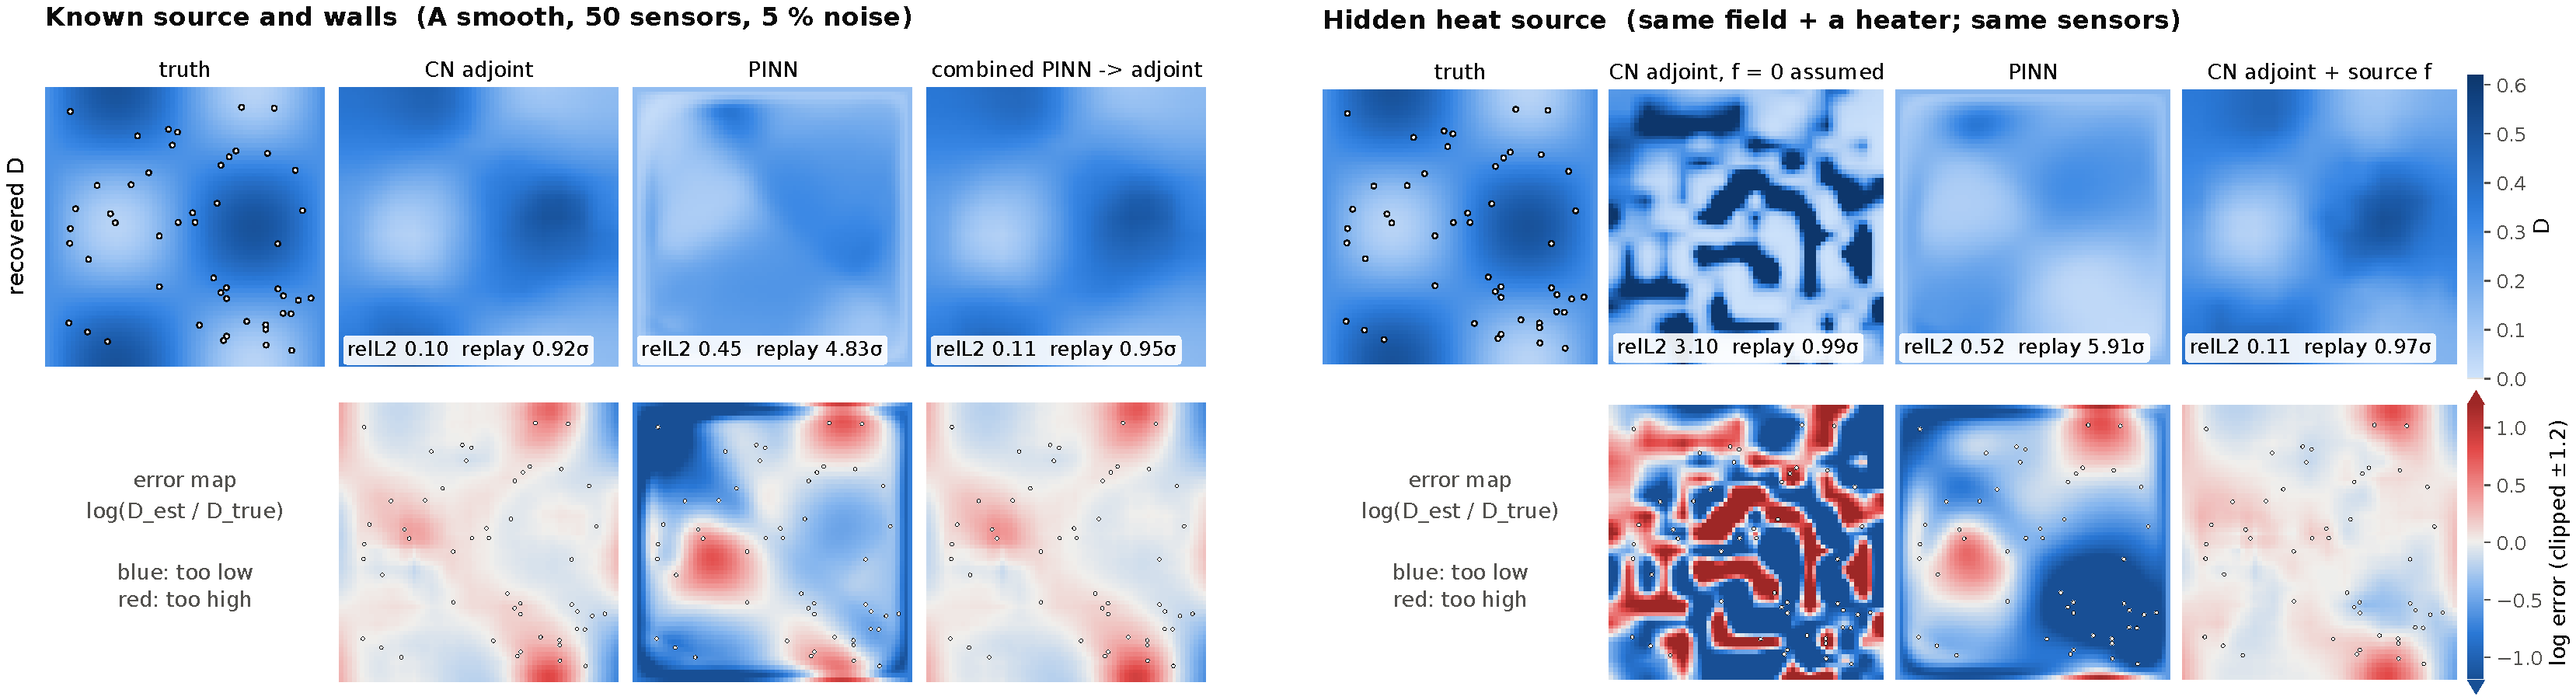
\includegraphics[width=\linewidth]{F12_fields_errors_replay.pdf}
\captionof{figure}{True and recovered $D$ with spatial error maps $\log(\hat D/D)$ and replay, same 50 sensors (dots).
Right: the adjoint that assumes no source fits the readings to $0.99\sigma$ with a wrong field.}
\end{minipage}\par\vspace{4pt}
\vspace{-6pt}
\begin{itemize}
\item \textbf{PINN vs CN adjoint, known physics.} The adjoint is about $2\times$ more accurate and explains the data
to the noise level; the PINN does not (median replay $3.6\sigma$, range 1.2 to over $100\sigma$). Over 5 seeds the
PINN beats the adjoint in only 3 of 100 dataset--seed pairs, all on one inclusion dataset. Seed 42 was the PINN's best
seed; its seed-to-seed spread is about 0.06.
\item \textbf{Combined method vs both standalone methods.} It always beats the PINN, but it does not beat the
adjoint: started from the PINN or from a constant, the adjoint ends at the same final $\alpha$ on 20 of 20 datasets,
because the strongly regularised start of the $\alpha$ path pulls any start to the same field. hybrid\_balance is
nearly seed-proof (0.223--0.228 vs the adjoint's 0.226) and beats both parents consistently (at least 4 of 5 seeds)
on 4 of 20 sharp-featured or noisy datasets. Using the PINN as a prior hurts (0.323); the reverse coupling
(adjoint$\to$PINN, 0.476) is no better than the PINN. Cost: about $3\times$ the adjoint alone, since our 2-D adjoint is cheap ($\approx37$\,s).
\item \textbf{Unknown physics.} An adjoint enforcing the wrong PDE must bend $D$ to explain heat it cannot account for
(errors 3--6), so the soft-physics PINN wins. Once the missing walls or source are estimated jointly, the classical
method wins again on 7 of 8 and 6 of 6 datasets, close to the true-physics bound. The PINN's real advantage is
producing a usable field without being told what physics is missing.
\item \textbf{Fit is not recovery.} With the hidden source the adjoint replays the sensors at $0.99\sigma$ yet has
rel$L_2$ 3.29: replay checks consistency with the data, not identification of $D$, so the full field and error map
must always be inspected.
\item \textbf{Controlled solver comparison.} BE is worse than CN in 8 of 9 noise/density cells (3\,969 sensors, 1\,\%
noise: 0.074 vs 0.046); CN with 100 steps matches a 4\,800-step reference. Mechanism: a BE step damps a mode by
$1/(1+x)$ instead of $e^{-x}$, so BE decays too slowly and mimics a smaller $D$; its temperature error is only
2.9\,\% of the signal but $2.5\sigma$ at 1\,\% noise, and since a 1\,\% change in $D$ moves $u$ by only 0.8\,\%, the
inversion inflates $D$ (higher than CN in 9 of 9 cells) and invents structure. Causal test: on BE-generated data BE
inverts as well as CN (0.093/0.093, 0.053/0.051, 0.047/0.046, 0.060/0.059). The intensive-phase ``PINN wins at high
density'' was this artefact; against CN the PINN reaches 0.384 on the same data (0.132 after 16$\times$ longer training).
\item \textbf{Sensor density.} From 20 to 3\,969 sensors (1\,\% noise) the PINN improves only from 0.481 to 0.404, the
adjoint from 0.156 to 0.070. Given the exact $u$, the PINN's $D$-step reaches 0.094 instead of 0.384: the PINN is limited
by fitting and differentiating its own $\hat u$, not by data.
\item \textbf{PINN improvements and model error.} Held-out validation picked a better model on 7 of 8 datasets; RAR
was worse on 8 of 8 (a large residual marks where $D$ is wrong, not a hard region of $u$); a learned $g(u)$ was worse on
4 of 6 and invented temperature dependence; pseudo-data wrecked the adjoint (0.317 $\to$ 3.38). With Arrhenius model
error the adjoint still won on 14 of 16 datasets; the PINN won only at strong dependence ($S=2$) with dense, clean data.
\end{itemize}

\section{Conclusions}
On matched data with the physics specified, the CN adjoint is the more accurate and better-calibrated method; the
combined method matches it but does not improve on it in our cheap 2-D setting. All three apparent PINN wins are
explained: a time integrator whose error exceeded the noise, unestimated walls and an unestimated source. The PINN
remains useful as a model-tolerant first look when the physics is uncertain. Future work: uncertain initial states,
3-D problems where an adjoint is expensive and a PINN warm start could pay off, and real thermography data.

{\footnotesize
\textbf{References.}
[1]~Maziar Raissi, Paris Perdikaris and George Em Karniadakis. Physics-informed neural networks: A deep learning
framework for solving forward and inverse problems involving nonlinear partial differential equations, Journal of
Computational Physics, 2019. \url{https://doi.org/10.1016/j.jcp.2018.10.045}
[2]~Zhen Zhang, Alessandro Alla and George Em Karniadakis. Adjoint Method versus Physics-Informed Neural Networks in
PDE-Constrained Inverse Problems, arXiv preprint, 2026. \url{https://arxiv.org/abs/2606.12337}
[3]~Sukirt Thakur, Ehsan Esmaili, Sarah Libring, Luis Solorio and Arezoo M. Ardekani. Inverse resolution of spatially
varying diffusion coefficient using physics-informed neural networks, Physics of Fluids, 2024.
\url{https://doi.org/10.1063/5.0207453}
\par}
\end{document}
